%%experimentos
\subsection{Resultados sobre datos artificiales}
\begin{frame}[t]
	\begin{scriptsize}
			\vspace{-2.7mm}
		\begin{block}{{Experimentos extremos sobre datos artificiales}}
			\begin{center}
			
%%%%%%%%%
% Table 1
\begin{table}
\label{table:extreme}
\smallskip\noindent
\scalebox{0.8}{
\begin{tabular}{ c | c | c  | c | c | c | c }
		& \multicolumn{2}{c|}{Soluciones} & \multicolumn{4}{c}{Índices} \\
		&$ C $ & $C^\prime$ & 
		\parbox[c][1em][c]{3em}{\begin{center} \textbf{FM} \end{center}} & 
		\parbox[c][1em][c]{3em}{\begin{center} \textbf{ARI} \end{center}} & 
		\parbox[c][1em][c]{3em}{\begin{center} \textbf{JAC}  \end{center}} & 
		\parbox[c][1em][c]{3em}{\begin{center} \textbf{\paperindex} \end{center}} \\ 
		\noalign{\smallskip}\noalign{\smallskip}\hline		
		\parbox[c][\alto{}][c]{3em}{\RNum{1}}
		&\parbox[c][\alto{}][c]{\ancho{}}{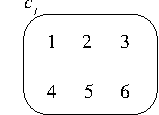
\includegraphics[scale=0.70]{{../figs/t11a}.pdf}} & %1
		\parbox[c][\alto{}][c]{\ancho{}}{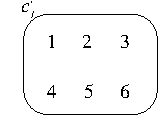
\includegraphics[scale=0.70]{{../figs/t11b}.pdf}}
		 &1.000  &--- &1.000  &1.000 		\\
		\parbox[c][\alto{}][c]{3em}{\RNum{2}}
		&\parbox[c][\alto{}][c]{\ancho{}}{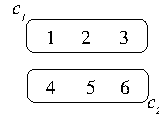
\includegraphics[scale=0.75]{{../figs/t12a}.pdf}} & %2
		\parbox[c][\alto{}][c]{\ancho{}}{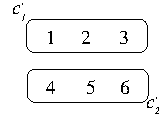
\includegraphics[scale=0.75]{{../figs/t12b}.pdf}}
		 &1.000  &1.000  &1.000  &1.000  		\\
		\parbox[c][\alto{}][c]{3em}{\RNum{3}}
		&\parbox[c][\alto{}][c]{\ancho{}}{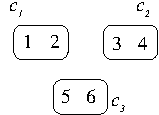
\includegraphics[scale=0.75]{{../figs/t13a}.pdf}} & %3
		\parbox[c][\alto{}][c]{\ancho{}}{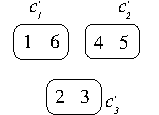
\includegraphics[scale=0.75]{{../figs/t13b}.pdf}}
		 &0.000  &-0.250  &0.000  &0.000	\\
		\parbox[c][\alto{}][c]{3em}{\RNum{4}}
		&\parbox[c][\alto{}][c]{\ancho{}}{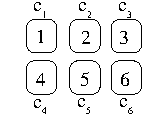
\includegraphics[scale=0.75]{{../figs/t14a}.pdf}} & %4
		\parbox[c][\alto{}][c]{\ancho{}}{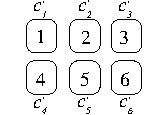
\includegraphics[scale=0.75]{{../figs/t14b}.pdf}}
		 &0.000  &---  &---  &0.000 		\\
	\end{tabular}
}	
\end{table}
%%%%%%%%%
	\end{center}		
	\end{block}
\end{scriptsize}
\end{frame}

\begin{frame}[t]
	\begin{scriptsize}
			\vspace{-2.7mm}
		\begin{block}{{Experimentos sobre datos artificiales con solapamiento gradual}}
			\begin{center}
%%%%%%%%%
% Table 2
\begin{table}
\scalebox{0.8}{
\begin{tabular}{ c | c | c  | c | c | c | c }
		& \multicolumn{2}{c|}{Soluciones} & \multicolumn{4}{c}{Índices} \\
		&$ C $ & $C^\prime$ & 
		\parbox[c][1em][c]{3em}{\begin{center} \textbf{FM} \end{center}} & 
		\parbox[c][1em][c]{3em}{\begin{center} \textbf{ARI} \end{center}} & 
		\parbox[c][1em][c]{3em}{\begin{center} \textbf{JAC}  \end{center}} & 
		\parbox[c][1em][c]{3em}{\begin{center} \textbf{\paperindex} \end{center}} \\ 
		\noalign{\smallskip}\hline\noalign{\smallskip}		
				\parbox[c][\alto{}][c]{3em}{\RNum{1}}
		&\parbox[c][\alto{}][c]{\ancho{}}{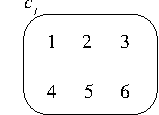
\includegraphics[scale=0.650]{{../figs/t21-6a}.pdf}} & %1
		\parbox[c][\alto{}][c]{\ancho{}}{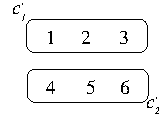
\includegraphics[scale=0.750]{{../figs/t12b}.pdf}}
		 &0.632  &0.000  &0.400  &0.400 		\\
		\parbox[c][\alto{}][c]{3em}{\RNum{2}}
		&\parbox[c][\alto{}][c]{\ancho{}}{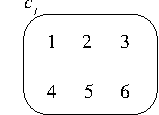
\includegraphics[scale=0.650]{{../figs/t21-6a}.pdf}} & %2
		\parbox[c][\alto{}][c]{\ancho{}}{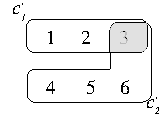
\includegraphics[scale=0.750]{{../figs/t22b}.pdf}}
		 &0.665  &-2.186  &0.442  &0.514 		\\
		\parbox[c][\alto{}][c]{3em}{\RNum{3}}
		&\parbox[c][\alto{}][c]{\ancho{}}{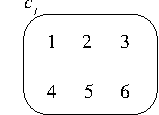
\includegraphics[scale=0.650]{{../figs/t21-6a}.pdf}} & %3
		\parbox[c][\alto{}][c]{\ancho{}}{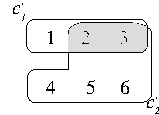
\includegraphics[scale=0.750]{{../figs/t23b_2}.pdf}}
		 &0.695  &2.347  &0.483  &0.650 		\\
		\parbox[c][\alto{}][c]{3em}{\RNum{4}}
		&\parbox[c][\alto{}][c]{\ancho{}}{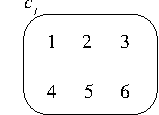
\includegraphics[scale=0.650]{{../figs/t21-6a}.pdf}} & %4
		\parbox[c][\alto{}][c]{\ancho{}}{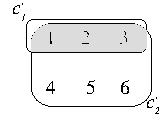
\includegraphics[scale=0.750]{{../figs/t24b_2}.pdf}}
		 &0.721   &1.444  &0.520  & 0.800 		\\
	\end{tabular}
}	
\end{table}
	\end{center}		
	\end{block}
\end{scriptsize}
\end{frame}

%%%%%%%%%%%%
\begin{frame}[t]
	\begin{scriptsize}
			\vspace{-2.7mm}
		\begin{block}{{Experimentos sobre datos artificiales con solapamiento gradual -- continuación}}
			\begin{center}
			%%%%%%%%%
% Table 2 continuación
\begin{table}
\scalebox{0.8}{
\begin{tabular}{ c | c | c  | c | c | c | c }
		& \multicolumn{2}{c|}{Soluciones} & \multicolumn{4}{c}{Índices} \\
		&$ C $ & $C^\prime$ & 
		\parbox[c][1em][c]{3em}{\begin{center} \textbf{FM} \end{center}} & 
		\parbox[c][1em][c]{3em}{\begin{center} \textbf{ARI} \end{center}} & 
		\parbox[c][1em][c]{3em}{\begin{center} \textbf{JAC}  \end{center}} & 
		\parbox[c][1em][c]{3em}{\begin{center} \textbf{\paperindex} \end{center}} \\ 
		\parbox[c][\alto{}][c]{3em}{\RNum{5}}
		&\parbox[c][\alto{}][c]{\ancho{}}{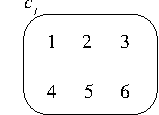
\includegraphics[scale=0.650]{{../figs/t21-6a}.pdf}} & %5
		\parbox[c][\alto{}][c]{\ancho{}}{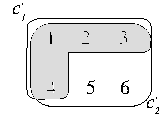
\includegraphics[scale=0.750]{{../figs/t25b_2}.pdf}}
		 &0.700  &1.324  &0.489  &0.840 		\\
		\parbox[c][\alto{}][c]{3em}{\RNum{6}}
		&\parbox[c][\alto{}][c]{\ancho{}}{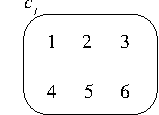
\includegraphics[scale=0.650]{{../figs/t21-6a}.pdf}} & %6
		\parbox[c][\alto{}][c]{\ancho{}}{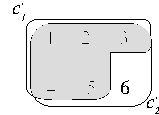
\includegraphics[scale=0.750]{{../figs/t26b_2}.pdf}}
		 &0.692  &1.238  &0.478  &0.909 		\\
		\parbox[c][\alto{}][c]{3em}{\RNum{7}}
		&\parbox[c][\alto{}][c]{\ancho{}}{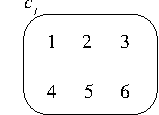
\includegraphics[scale=0.650]{{../figs/t21-6a}.pdf}} & %7
		\parbox[c][\alto{}][c]{\ancho{}}{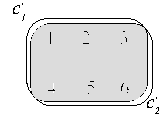
\includegraphics[scale=0.750]{{../figs/t27b_2}.pdf}}
		 &0.692  &1.179  &0.478  &1.000		\\
		\noalign{\smallskip}\hline
	\end{tabular}
}	
\end{table}
%%%%%%%%%
	\end{center}		
	\end{block}
\end{scriptsize}
\end{frame}
%%%%%%%%%%%%


\begin{frame}[t]
	\begin{scriptsize}
		\vspace{-2.7mm}
		\begin{block}{{Experimentos sobre datos artificiales con solapamiento extremo}}
			\begin{center}
%%%%%%%%%
% Table 3
\begin{table}
\scalebox{0.8}{
\begin{tabular}{ c | c | c  | c | c | c | c }
\hline\noalign{\smallskip}
		& \multicolumn{2}{c|}{Soluciones} & \multicolumn{4}{c}{Índices} \\
		&$ C $ & $C^\prime$ & 
		\parbox[c][1em][c]{3em}{\begin{center} \textbf{FM} \end{center}} & 
		\parbox[c][1em][c]{3em}{\begin{center} \textbf{ARI} \end{center}} & 
		\parbox[c][1em][c]{3em}{\begin{center} \textbf{JAC}  \end{center}} & 
		\parbox[c][1em][c]{3em}{\begin{center} \textbf{\paperindex} \end{center}} \\ 
		\noalign{\smallskip}\hline\noalign{\smallskip}		
		\parbox[c][\alto{}][c]{3em}{\RNum{1}}
		&\parbox[c][\alto{}][c]{\ancho{}}{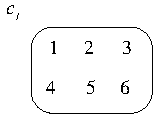
\includegraphics[scale=0.750]{{../figs/t31a}.pdf}} & %1
		\parbox[c][\alto{}][c]{\ancho{}}{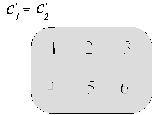
\includegraphics[scale=0.750]{{../figs/t31b_2}.pdf}}
		 &0.692  &1.179  &0.478  &1.000 		\\
		\parbox[c][\alto{}][c]{3em}{\RNum{2}}
		&\parbox[c][\alto{}][c]{\ancho{}}{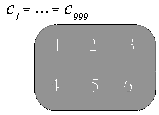
\includegraphics[scale=0.750]{{../figs/t33a_2}.pdf}} & %2
		\parbox[c][\alto{}][c]{\ancho{}}{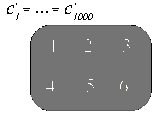
\includegraphics[scale=0.750]{{../figs/t33b_2}.pdf}}
		 &0.001  &1.000  &0.001  &1.000 		\\
		\parbox[c][\alto{}][c]{3em}{\RNum{3}}
		&\parbox[c][\alto{}][c]{\ancho{}}{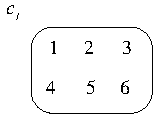
\includegraphics[scale=0.750]{{../figs/t34a}.pdf}} & %3
		\parbox[c][\alto{}][c]{\ancho{}}{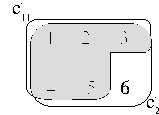
\includegraphics[scale=0.750]{{../figs/t34b_2}.pdf}}
		 &0.692  &1.238  &0.478  &0.909 		\\
		\parbox[c][\alto{}][c]{3em}{\RNum{4}}
		&\parbox[c][\alto{}][c]{\ancho{}}{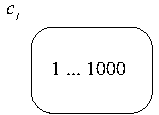
\includegraphics[scale=0.750]{{../figs/t35a}.pdf}} & %4
		\parbox[c][\alto{}][c]{\ancho{}}{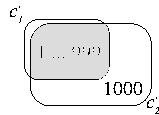
\includegraphics[scale=0.750]{{../figs/t35b_2}.pdf}}
		 &0.707  &1.200  &0.500  &0.999 		\\
		\noalign{\smallskip}\hline
	\end{tabular}
}	
\end{table}
%%%%%%%%%
	\end{center}		
	\end{block}
\end{scriptsize}
\end{frame}

\subsection{Resultados sobre bases de datos reales}
\begin{frame}
	\begin{block}{Experimentos sobre BDs reales -- Parámetros}
			\visible<1-> {Se utilizaron las BD de Iris, Yeast, Glass, Wine} \\
			\visible<2-> {Se realizó clustering con Mapas auto--organizativos (SOM)}\\
			\visible<3-> {Solapamiento usando el concepto de vecindad solamente en las soluciones $C^\prime$}\\
			\begin{tabular}{l r}
				\visible<3-> {Sin solapamiento: $V_n=0$ & 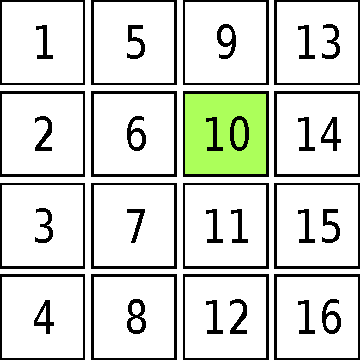
\includegraphics[scale=0.3]{./figs/figure_som_vn0.pdf}} \\
				\visible<4-> {Con solapamiento: $V_n=1$ & 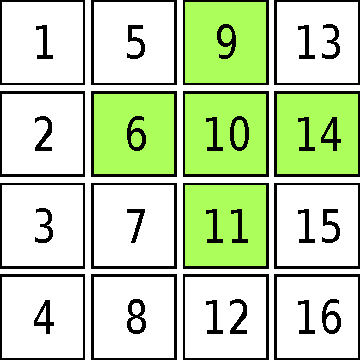
\includegraphics[scale=0.3]{./figs/figure_som_vn1.pdf}} \\		
			\end{tabular}\\
			\smallskip
			\visible<5-> { En todos los casos las soluciones $C$ se consideraron sin solapamiento ($V_n=0$)}\\			

	\end{block}		
\end{frame}

\begin{frame}[t]
\begin{flushleft}

%%%%%%%%%
% Table 4
\begin{scriptsize}
\hspace*{-3pt}\makebox[\linewidth][c]{%
\scalebox{0.84}{
\begin{tabular}{c | c | c | c | c | c | c | c | c | c }
\hline\noalign{\smallskip}
  \multirow{2}{*}{} & \multirow{2}{*} { \textbf{clusters en $C$ y $C^\prime$}} & \multicolumn{2}{c|}{\textbf{FM}} & 	\multicolumn{2}{c|}{\textbf{ARI}} &	\multicolumn{2}{c|}{\textbf{JAC}} &	\multicolumn{2}{c}{\textbf{\paperindex}}\\
         & & \visible<1> {\textbf{$Vn=0$}}& \visible<2> {\textbf{$Vn=1$}}  & \visible<1> {\textbf{$Vn=0$}} & \visible<2> {\textbf{$Vn=1$}} & \visible<1> {\textbf{$Vn=0$}} & \visible<2> {\textbf{$Vn=1$}}& \visible<1> {\textbf{$Vn=0$}} &\visible<2> { \textbf{$Vn=1$}}\\
		\noalign{\smallskip}\hline\noalign{\smallskip}		
        \multicolumn{5}{c}{} \\ %
        \multirow{3}{*}{Iris} & $k=4$ vs $k^{\prime}=25$  &  \visible<1> { $0.33}$ & \visible<2> {$0.30$} & \visible<1> {$0.16$} & \visible<2> {$4.26 $} & \visible<1> {$0.14$} & \visible<2> {$0.10$} & \visible<1> {$0.14$} & \visible<2> {$0.38$} \\
        &$k=4$ vs $k^{\prime}=100$  &  \visible<1> {$ 0.17 } $  & \visible<2> {$ 0.16$}  & \visible<1> {$ 0.03$} & \visible<2> {$-0.66$}& \visible<1> {$0.03$}& \visible<2> {$0.03$}& \visible<1> {$0.03$}& \visible<2> {$0.11$}\\
        \cdashline{2-10}[0.5pt/1pt]
        &$k=25$ vs $k^{\prime}=100$  & \visible<1> {$ 0.33$}  & \visible<2> {$	0.23 $ } & \visible<1> {$ 0.23 $} &\visible<2> { $	-0.34$} & \visible<1> {$0.14$}& \visible<2> {$0.09$}& \visible<1> {$0.14$}& \visible<2> {$0.37$}\\
        \hline\hline        
        \multicolumn{5}{c}{} \\ %
		\end{tabular}	
}		
}	
\end{scriptsize}		
			\begin{tabular}{l r}
				\only<1> {Sin solapamiento: $V_n=0$ & 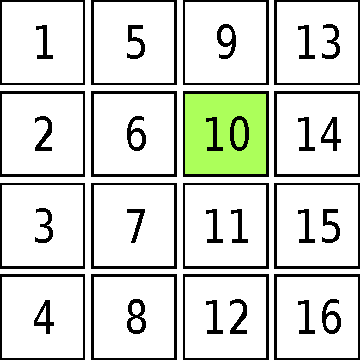
\includegraphics[scale=0.4]{./figs/figure_som_vn0.pdf}} \\
				\only<2> {Con solapamiento: $V_n=1$ & 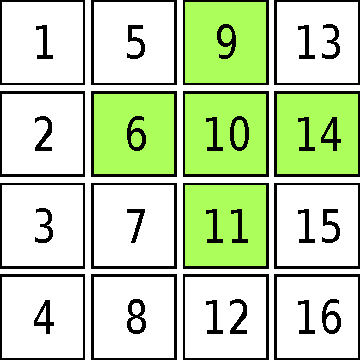
\includegraphics[scale=0.4]{./figs/figure_som_vn1.pdf}} \\		
			\end{tabular} 
			\end{flushleft}		
\end{frame}


\begin{frame}
\begin{flushleft}
%%%%%%%%%
% Table 4
\vspace{-28mm}
\begin{scriptsize}
\hspace*{-3pt}\makebox[\linewidth][c]{%
\scalebox{0.84}{
\begin{tabular}{c | c | c | c | c | c | c | c | c | c }
\hline\noalign{\smallskip}
  \multirow{2}{*}{} & \multirow{2}{*} { \textbf{clusters en $C$ y $C^\prime$}} & \multicolumn{2}{c|}{\textbf{FM}} & 	\multicolumn{2}{c|}{\textbf{ARI}} &	\multicolumn{2}{c|}{\textbf{JAC}} &	\multicolumn{2}{c}{\textbf{\paperindex}}\\
         & & \textbf{$Vn=0$} & \textbf{$Vn=1$}  & \textbf{$Vn=0$} & \textbf{$Vn=1$} & \textbf{$Vn=0$} & \textbf{$Vn=1$}& \textbf{$Vn=0$} & \textbf{$Vn=1$}\\
		\noalign{\smallskip}\hline\noalign{\smallskip}		
        \multicolumn{5}{c}{} \\ %
        \multirow{3}{*}{Iris} & $k=4$ vs $k^{\prime}=25$  &   $0.33$ & $0.30$ & $0.16$ & $4.26 $ & $0.14$ & $0.10$& $0.14$& $0.38$ \\
        &$k=4$ vs $k^{\prime}=100$  &  $ 0.17  $  & $ 0.16$  & $ 0.03$ & $-0.66$& $0.03$& $0.03$& $0.03$& $0.11$\\
        \cdashline{2-10}[0.5pt/1pt]
        &$k=25$ vs $k^{\prime}=100$  & $ 0.33$  & $	0.23 $  & $ 0.23 	 $ & $	-0.34$ & $0.14$& $0.09$& $0.14$& $0.37$\\
        \hline\hline        
        \multicolumn{5}{c}{} \\ %
        %\end of Iris                                   
		\end{tabular}	
}		
}	
\end{scriptsize}		

			\end{flushleft}		
\end{frame}

\begin{frame}
\begin{flushleft}
%%%%%%%%%
% Table 4
\begin{scriptsize}
\hspace*{-3pt}\makebox[\linewidth][c]{%
\scalebox{0.84}{
\begin{tabular}{c | c | c | c | c | c | c | c | c | c }
\hline\noalign{\smallskip}
  \multirow{2}{*}{} & \multirow{2}{*} { \textbf{clusters en $C$ y $C^\prime$}} & \multicolumn{2}{c|}{\textbf{FM}} & 	\multicolumn{2}{c|}{\textbf{ARI}} &	\multicolumn{2}{c|}{\textbf{JAC}} &	\multicolumn{2}{c}{\textbf{\paperindex}}\\
         & & \textbf{$Vn=0$} & \textbf{$Vn=1$}  & \textbf{$Vn=0$} & \textbf{$Vn=1$} & \textbf{$Vn=0$} & \textbf{$Vn=1$}& \textbf{$Vn=0$} & \textbf{$Vn=1$}\\
		\noalign{\smallskip}\hline\noalign{\smallskip}		
        \multicolumn{5}{c}{} \\ %
        \multirow{3}{*}{Iris} & $k=4$ vs $k^{\prime}=25$  &   $0.33$ & $0.30$ & $0.16$ & $4.26 $ & $0.14$ & $0.10$& $0.14$& $0.38$ \\
        &$k=4$ vs $k^{\prime}=100$  &  $ 0.17  $  & $ 0.16$  & $ 0.03$ & $-0.66$& $0.03$& $0.03$& $0.03$& $0.11$\\
        \cdashline{2-10}[0.5pt/1pt]
        &$k=25$ vs $k^{\prime}=100$  & $ 0.33$  & $	0.23 $  & $ 0.23 	 $ & $	-0.34$ & $0.14$& $0.09$& $0.14$& $0.37$\\
        \hline\hline        
        \multicolumn{5}{c}{} \\ %
        %\end Iris                                   
        \multirow{3}{*}{Wine} & $k=4$ vs $k^{\prime}=25$  &   $0.40$ & $0.32$ & $0.23$ & $9.33 $ & $0.17$& $0.12$& $0.17$& $0.48$\\
        &$k=4$ vs $k^{\prime}=100$  &  $ 0.19  $  & $ 0.18$  & $ 0.06$ & $-0.52$& $0.04$& $0.04$& $0.04$& $0.14$\\
        \cdashline{2-10}[0.4pt/1pt]
        &$k=25$ vs $k^{\prime}=100$  & $ 0.34$  & $	0.23 $  & $ 0.26 	 $ & $	-0.24$ & $0.15$& $0.10$& $0.17$& $0.39$\\
        \hline\hline
        \multicolumn{5}{c}{} \\ %        
         %\end wine     
        \multirow{3}{*}{Yeast} & $k=4$ vs $k^{\prime}=25$  &   $0.32$ & $0.23$ & $0.15$ & $6.61 $  & $0.13$& $0.08$& $0.13$& $0.35$\\
        &$k=4$ vs $k^{\prime}=100$  &  $ 0.16  $  & $ 0.14$  & $ 0.04$ & $-0.58$& $0.03$& $0.03$& $0.03$& $0.11$\\
        \cdashline{2-10}[0.5pt/1pt]
        &$k=25$ vs $k^{\prime}=100$  & $ 0.29$  & $	0.18 $  & $ 0.21 	 $ & $-0.30$ & $0.13$& $0.07$& $0.14$& $0.33$\\
        \hline\hline
        \multicolumn{5}{c}{} \\ %              
         %\end Yeast             
        \multirow{3}{*}{Glass} & $k=4$ vs $k^{\prime}=25$  &  $0.33$ & $0.27$ & $0.10$ & $3.77 $ & $0.11$ & $0.08$& $0.11$& $0.30$ \\
        &$k=4$ vs $k^{\prime}=100$  &  $ 0.15  $  & $ 0.14$  & $ 0.02$ & $-0.75$& $0.02$& $0.02$& $0.02$& $0.09$\\
        \cdashline{2-10}[0.5pt/1pt]
        &$k=25$ vs $k^{\prime}=100$  & $ 0.38$  & $	0.24$  & $0.28 	 $ & $	-0.36$ & $0.17$& $0.09$& $0.18$& $0.43$\\
        \hline\hline
        \multicolumn{5}{c}{} \\ %              
         %\end of Glass         
		\noalign{\smallskip}\hline		
		\end{tabular}	
}		
}	
\end{scriptsize}		
\end{flushleft}		
\end{frame}


\subsection{Resultados sobre una red social: YouTube}
\begin{frame}[t]
	\begin{block}{Cojunto de datos YouTube}
		\begin{itemize}
			\item<1-> Cada línea del conjunto de datos posee los IDs de usurios que forman una comunidad con intereses en común
			\item<2-> Un usuario puede pertenecer a más de una comunidad
			\item<3-> Una comunidad se dice solapada si tiene al menos un usuario que pertenezca también a otra comunidad
			\item<4-> El nivel de solpamiento de una comunidad depende de la cantidad de sus participantes que pertenezcan a otras comunidades.
		\end{itemize}
	\end{block}
\end{frame}


\begin{frame}[t]

	\begin{block}{Experimento}
		\begin{itemize}
			\item<1-> Para la solución de referencia ($C$) se ordenaron los grupos por grado de solapamiento
			\item<2-> La solución comparativa ($C^\prime$) si tomó de $C$, y se le aplicaron modificaciones aleatorias
			\item<3-> En $C^\prime$, se agregó un $10\%$ de usuarios a distintas comunidades
			\item<4-> Las primeras $35$ comunidades forman el grupo de las comunidades \textbf{sin solapamiento}
			\item<5-> Las demás comunidades se dividieron en $16$ grupos en \textbf{orden creciente} de solapamiento.
		\end{itemize}
	\end{block}
\end{frame}

\begin{frame}[t]
\vspace{-4mm}
	\begin{scriptsize}
		\begin{center}
			{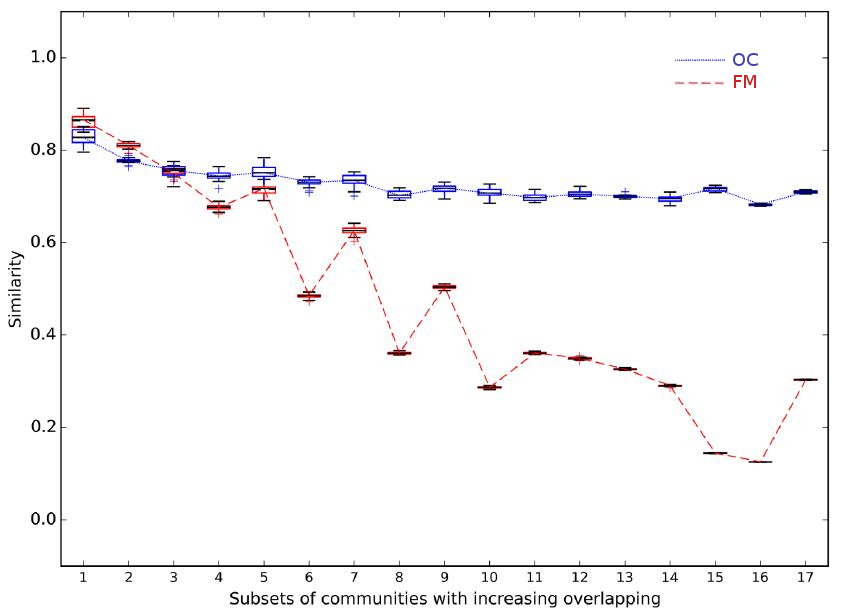
\includegraphics[scale=0.48]{{../figs/rt5_1}.jpg}}
		\end{center}		
	\end{scriptsize}
\end{frame}

\subsection{Publicaciones}
\begin{frame}[t]
		\begin{block}{{Publicaciones realizadas durante el doctorado}}
			\begin{center}
				\begin{itemize}
					\item  {Campo, D., Stegmayer, G., Milone, D.: A new index for clustering validation with overlapped
clusters. Expert Systems with Applications (\textbf{en revisión})} 		
					\item  Campo, D., Stegmayer, G., Milone, D.: Stability analysis in overlapped clusters. Iberoamerican
Journal of Artificial Intelligence 17(53) (2014) 79–89 
					\item  Campo, David; Stegmayer, Georgina; Milone Diego, ``Nuevo índice para el análisis de
estabilidad en clusters solapados'', Simposio Argentino de Inteligencia Artificial. 42 Jornadas
Argentinas de Informática, ISSN: 1850–2784. Pages: 24–35.
Córdoba, Argentina
				\end{itemize}
			\end{center}		
		\end{block}
\end{frame}
